\documentclass[journal,12pt,twocolumn]{IEEEtran}
\usepackage{setspace}
\usepackage{gensymb}
\singlespacing
\usepackage[cmex10]{amsmath}
\usepackage{amsthm}
\usepackage{amsmath}
\usepackage{mathrsfs}
\usepackage{txfonts}
\usepackage{stfloats}
\usepackage{bm}
\usepackage{cite}
\usepackage{cases}
\usepackage{subfig}
\usepackage{longtable}
\usepackage{multirow}
\usepackage{enumitem}
\usepackage{mathtools}
\usepackage{steinmetz}
\usepackage{tikz}
\usepackage{circuitikz}
\usepackage{verbatim}
\usepackage{tfrupee}
\usepackage[breaklinks=true]{hyperref}
\usepackage{graphicx}
\usepackage{tkz-euclide}
\usetikzlibrary{calc,math}
\usepackage{listings}
\usepackage{color}                                            %%
\usepackage{array}                                            %%
\usepackage{longtable}                                        %%
\usepackage{calc}                                             %%
\usepackage{multirow}                                         %%
\usepackage{hhline}                                           %%
\usepackage{ifthen}                                           %%
\usepackage{lscape}     
\usepackage{multicol}
\usepackage{chngcntr}
\DeclareMathOperator*{\Res}{Res}
\renewcommand\thesection{\arabic{section}}
\renewcommand\thesubsection{\thesection.\arabic{subsection}}
\renewcommand\thesubsubsection{\thesubsection.\arabic{subsubsection}}
\renewcommand\thesectiondis{\arabic{section}}
\renewcommand\thesubsectiondis{\thesectiondis.\arabic{subsection}}
\renewcommand\thesubsubsectiondis{\thesubsectiondis.\arabic{subsubsection}}
\hyphenation{op-tical net-works semi-conduc-tor}
\def\inputGnumericTable{}                                 %%

\lstset{
%language=C,
frame=single, 
breaklines=true,
columns=fullflexible
}

\begin{document}
\newtheorem{theorem}{Theorem}[section]
\newtheorem{problem}{Problem}
\newtheorem{proposition}{Proposition}[section]
\newtheorem{lemma}{Lemma}[section]
\newtheorem{corollary}[theorem]{Corollary}
\newtheorem{example}{Example}[section]
\newtheorem{definition}[problem]{Definition}
\newcommand{\BEQA}{\begin{eqnarray}}
\newcommand{\EEQA}{\end{eqnarray}}
\newcommand{\define}{\stackrel{\triangle}{=}}
\bibliographystyle{IEEEtran}
\raggedbottom
\setlength{\parindent}{0pt}
\providecommand{\mbf}{\mathbf}
\providecommand{\pr}[1]{\ensuremath{\Pr\left(#1\right)}}
\providecommand{\qfunc}[1]{\ensuremath{Q\left(#1\right)}}
\providecommand{\sbrak}[1]{\ensuremath{{}\left[#1\right]}}
\providecommand{\lsbrak}[1]{\ensuremath{{}\left[#1\right.}}
\providecommand{\rsbrak}[1]{\ensuremath{{}\left.#1\right]}}
\providecommand{\brak}[1]{\ensuremath{\left(#1\right)}}
\providecommand{\lbrak}[1]{\ensuremath{\left(#1\right.}}
\providecommand{\rbrak}[1]{\ensuremath{\left.#1\right)}}
\providecommand{\cbrak}[1]{\ensuremath{\left\{#1\right\}}}
\providecommand{\lcbrak}[1]{\ensuremath{\left\{#1\right.}}
\providecommand{\rcbrak}[1]{\ensuremath{\left.#1\right\}}}
\theoremstyle{remark}
\newtheorem{rem}{Remark}
\newcommand{\sgn}{\mathop{\mathrm{sgn}}}
%\providecommand{\abs}[1]{\left\vert#1\right\vert}
\providecommand{\res}[1]{\Res\displaylimits_{#1}} 
\providecommand{\norm}[1]{$\left\lVert#1\right\rVert$}
%\providecommand{\norm}[1]{\lVert#1\rVert}
\providecommand{\mtx}[1]{\mathbf{#1}}
\providecommand{\mean}[1]{E$\left[ #1 \right]$}
\providecommand{\fourier}{\overset{\mathcal{F}}{ \rightleftharpoons}}
%\providecommand{\hilbert}{\overset{\mathcal{H}}{ \rightleftharpoons}}
\providecommand{\system}{\overset{\mathcal{H}}{ \longleftrightarrow}}
%\newcommand{\solution}[2]{\textbf{Solution:}{#1}}
\newcommand{\solution}{\noindent \textbf{Solution: }}
\newcommand{\cosec}{\,\text{cosec}\,}
\providecommand{\dec}[2]{\ensuremath{\overset{#1}{\underset{#2}{\gtrless}}}}
\newcommand{\myvec}[1]{\ensuremath{\begin{pmatrix}#1\end{pmatrix}}}
\newcommand{\mydet}[1]{\ensuremath{\begin{vmatrix}#1\end{vmatrix}}}
\numberwithin{equation}{subsection}
\makeatletter
\@addtoreset{figure}{problem}
\makeatother
\let\StandardTheFigure\thefigure
\let\vec\mathbf
\renewcommand{\thefigure}{\theproblem}
\def\putbox#1#2#3{\makebox[0in][l]{\makebox[#1][l]{}\raisebox{\baselineskip}[0in][0in]{\raisebox{#2}[0in][0in]{#3}}}}
\def\rightbox#1{\makebox[0in][r]{#1}}
\def\centbox#1{\makebox[0in]{#1}}
\def\topbox#1{\raisebox{-\baselineskip}[0in][0in]{#1}}
\def\midbox#1{\raisebox{-0.5\baselineskip}[0in][0in]{#1}}

\title{EE3015 - IDP}
\author{Krishna Chaitanya \\
EE17BTECH11028}
\maketitle
\newpage
\medskip
\renewcommand{\thefigure}{\theenumi}
\renewcommand{\thetable}{\theenumi}
All codes available at
\begin{lstlisting}
https://github.com/EE17BTECH11028/EE3015.git
\end{lstlisting}

\section{Question 5.3 in gvv\_filter.pdf}
\medskip 
The system h(n) is said to be stable if 
\begin{align}
     \sum_{n=-\infty}^{\infty} \abs{|h(n)|} < \infty
\end{align} 
Is the system defined by 
\begin{align}
    y(n)+\frac{1}{2}y(n-1) = x(n)+x(n-2) 
\end{align}
with  
\begin{align}
      y(n)=0 \text{ for }n<0
\end{align}
stable for impulse response defined using the\\ $Z-transform$, 
\begin{align}
    H(z) = \frac{Y(z)}{X(z)}
\end{align}
?
\section{Solution}
We can verify the stability through\\ 1. Bounded Input - Bounded Output(BIBO) stability \\ 2. pole-zero plot. 
\section{BIBO stability}
 A system is said to be BIBO stable, if the output of the system is bounded for every input to the system that is bounded.
\begin{align}
    |x(n)|\leq B_x \implies |y(n)| \leq B_y
\end{align}
where
\begin{align}
    B_x < \infty \\ B_y < \infty
\end{align}

Let the input $x(n)$ be bounded, \\
\begin{align}
    |x(n)|\leq B_x<\infty
\end{align}
For a given $x(n), y(n)$ is defined as
\begin{align}
    y(n)=\sum_{-\infty}^{\infty}h(k)\,x(n-k)
\end{align}
where h(k) is the impulse function\bigskip\\ 
Considering the modulus of the equation\\
\begin{align}
    |y(n)|=|\sum_{-\infty}^{\infty}h(k)\,x(n-k)\,|
\end{align}
Replacing the value of x(n) with it's maximum value $B_x$ to obtain the bounds of y(n)
\begin{align}
    \implies |y(n)| \leq |\sum_{-\infty}^{\infty}h(k)\,B_x\,|\\
    \implies |y(n)| \leq B_x\,|\sum_{-\infty}^{\infty}h(k)\,|
\end{align}
For the system to be BIBO stable, $|y(n)| < \infty$. This holds only if 
\begin{align}
    |y(n)| < \infty
\end{align}
\begin{align}
    \implies |\sum_{-\infty}^{\infty}h(k)\,| < \infty
\end{align}
since $B_x$ is known to be a finite value\medskip \\
So for the system to be BIBO stable, it's impulse response in time domain must be absolutely summable to a finite value.\bigskip  

\section{Impulse response}
For the given system,
\begin{align}
    y(n)+\frac{1}{2}y(n-1) = x(n)+x(n-2) \\
    y(n)=0 \text{ for }n<0
\end{align}
Apply Z-transform on both sides,
\begin{align}
    Y(z) + \frac{1}{2}z^{-1}Y(z)=X(z) + z^{-2}X(z)\\
    \implies Y(z)=\frac{1+z^{-2}}{1+\frac{1}{2}z^{-1}}X(z)\\
    \implies \frac{Y(z)}{X(z)}=\frac{1+z^{-2}}{1+\frac{1}{2}z^{-1}}
\end{align}
We defined Z-transform of impulse to be 
\begin{align}
    H(z) = \frac{Y(z)}{X(z)}
\end{align}
So,
\begin{align}
    H(z) = \frac{1+z^{-2}}{1+\frac{1}{2}z^{-1}}\\
    \implies H(z) = \frac{1}{1+\frac{1}{2}z^{-1}} + \frac{z^{-2}}{1+\frac{1}{2}z^{-1}}
\end{align}
Applying $inverse Z-transform$ on both sides,
\begin{align}
\implies h(n)=\sbrak{\frac{-1}{2}}^nu(n) + \sbrak{\frac{-1}{2}}^{n-2}u(n-2)
\end{align}
Now that we have calculated the impulse response, let's verify it's BIBO stability by verifying if
\begin{align}
    |\sum_{-\infty}^{\infty}h(n)\,| < \infty 
\end{align}
\begin{align}
    |\sum_{-\infty}^{\infty}h(n)\,| =
    \sum_{n=-\infty}^{\infty}|\abs{\sbrak{\frac{-1}{2}}^nu(n) + \sbrak{\frac{-1}{2}}^{n-2}u(n-2)}| 
\end{align}
\begin{align}
    |\sum_{-\infty}^{\infty}h(n)\,| = \sum_{n=-\infty}^{\infty}|\abs{\sbrak{\frac{1}{2}}^nu(n) + \sbrak{\frac{1}{2}}^{n-2}u(n-2)}|
\end{align}
\\Since n is running from $-\infty$ to $\infty$, the time shift can be ignored
\begin{align}
    |\sum_{-\infty}^{\infty}h(n)\,| = 2\sum_{n=-\infty}^{\infty}|\abs{\sbrak{\frac{1}{2}}^nu(n)}|
\end{align}
\begin{align}
    |\sum_{-\infty}^{\infty}h(n)\,| = 2\sum_{n=0}^{\infty}{\sbrak{\frac{1}{2}}^n}
\end{align}
Using the sum of infinite length Geometric Progression,
\begin{align}
    |\sum_{-\infty}^{\infty}h(n)\,| = 2\sbrak{\frac{1}{1-\frac{1}{2}}} 
    = 4
\end{align}
As impulse response sums up to a finite value,
\begin{align}
|\sum_{-\infty}^{\infty}h(n)\,| < \infty
\end{align}
The system is BIBO stable.\\ 

\section{Pole-Zero Plot}
 We obtained Z-transform of the impulse response from the system as
\begin{align}
    H(z) = \frac{1+z^{-2}}{1+\frac{1}{2}z^{-1}} 
\end{align}
\begin{align}
    \implies H(z) = \frac{2(z^2+1)}{z(2z+1)} 
\end{align}
Solving for poles and zeros, we get, 
\begin{center}
    Poles = $0 , -\frac{1}{2}$ \medskip \\
    zeros = $+1j, -1j$
\end{center}

\begin{figure}[h!]
    \centering
    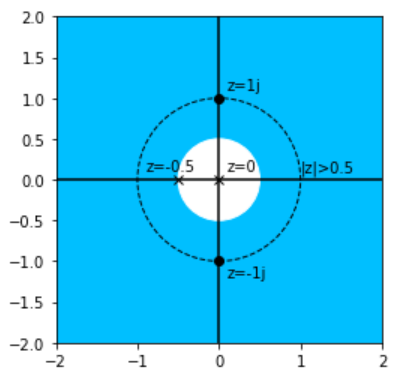
\includegraphics[scale=0.42]{polezero.png}
    \caption{Pole-Zero Plot}
\end{figure}

In the Pole-Zero plot, the poles of the impulse response lie in the left half of the s-plane which proves that the system is stable.\\

\textbf{Let's verify the stability of the system for input from 3.1, gvv\_filter.pdf} 
\medskip
Input is given as,
\begin{align}
    x(n)=\{1,2,3,4,2,1\}
\end{align}
\begin{align}
    y(n)+\frac{1}{2}y(n-1) = x(n)+x(n-2) \\
    y(n)=0 \text{ for }n<0
\end{align}

\begin{figure}[h!]
    \centering
    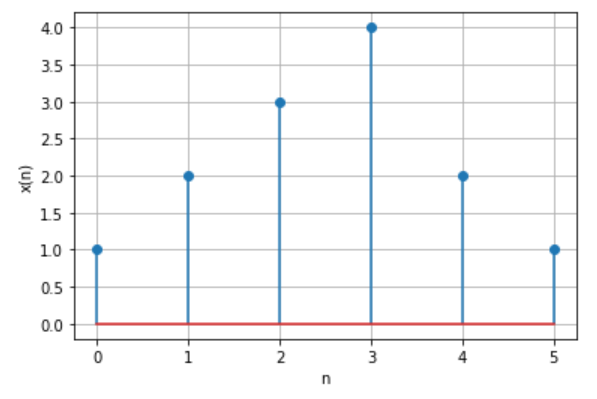
\includegraphics[scale=0.42]{input.png}
    \caption{Input signal, x(n)}\label{fig:df1a}
\end{figure}
From the above plot $B_x=4$ for the input signal. \medskip

\begin{figure}[h!]
    \centering
    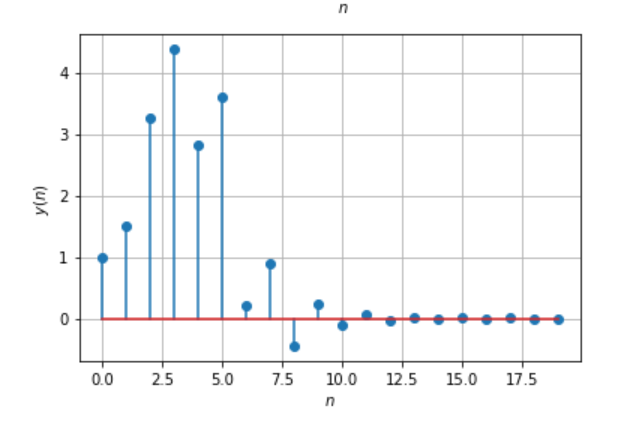
\includegraphics[scale=0.42]{output.png}
    \caption{Output signal, y(n)}
\end{figure}
From the above plot $B_y=4.375$ for the output signal.\medskip\\ Since the input and output are bounded, the system is stable.

\end{document}